\documentclass[aspectratio=43]{beamer}
\usepackage[latin1]{inputenc}
\usepackage{amsmath}
\usepackage{amsfonts}
\usepackage{amssymb}
\usepackage{makeidx}
\usepackage{graphicx}
\usepackage{array}
\usepackage{braket}

% Customization
\mode<presentation>{
\usetheme{CambridgeUS}
\usecolortheme{dolphin}
\setbeamertemplate{navigation symbols}{}
}

%\setbeamertemplate{footline}[frame number]

% Title and author
\title[QCD and Monte Carlo]{Quantum Coherent Phenomena}
\author{\textbf {Jes\'us Urtasun Elizari}}
%\institute{\textbf {University of Milan}}
\date{Milan, October 2020}

\begin{document}

% Front slide
\begin{frame}

	%\maketitle
	\vspace{1.0 cm}
	
	\center{\color{blue}Two-mode squeezed states in cavity optomechanics\\ via engineering of a single reservoir}
	
	\vspace{0.25 cm}
	\center{Quantum coherent phenomena course seminar - Milan, October 2020}

	\begin{figure}
		\minipage{1\textwidth}
		
\includegraphics[width = 3.0 cm]{plots/logo_unimi.png}
		\hfill
		
\includegraphics[width = 3.0 cm]{plots/logo_infn.png}
		\hfill
		
\includegraphics[width = 3.0 cm]{plots/logo_erc.png}
		\endminipage
	\end{figure}

	\vspace{1.0 cm}

\end{frame}

% Introduction
\begin{frame}

	\frametitle{Outline}
	
	\begin{enumerate}
		\item {\color{blue}Introduction, system and Hamiltonian}
		\item {\color{blue}Reservoir engineering strategies}
		\item {\color{blue}Implementation}
		\item {\color{blue}Full system}
		\item {\color{blue}Experimental observability}
		\item {\color{blue}Conclusions}
	\end{enumerate}
	
\end{frame}

% Introduction
\begin{frame}

	\frametitle{Introduction}
	\framesubtitle{Entangled states}

	\begin{enumerate}
		\item Generation and detection of entangled states of macroscopic M.O
		\item Reservoir engineering $\longrightarrow$ Two-mode squeezed states
		\item Easy to implement in existing experimental configurations
		\item Quantum optomechanics $\longrightarrow$ couple Bogoliubov modes to a single reservoir (damped cavity)
	\end{enumerate}	
	
\end{frame}

% System and Hamiltonian I
\begin{frame}

	\frametitle{Introduction}
	\framesubtitle{System representation}
	
	\begin{itemize}
		\item Two mechanical oscillators, resonance frequencies $\omega_{a}, \omega_{b}$
		\item Dispersively coupled $g_{a}, g_{b}$ to a common cavity $\omega_{c}$
		\item Dispersively coupled $g_{a}, g_{b}$ to a common cavity $\omega_{c}$
	\end{itemize}

		\begin{figure}
			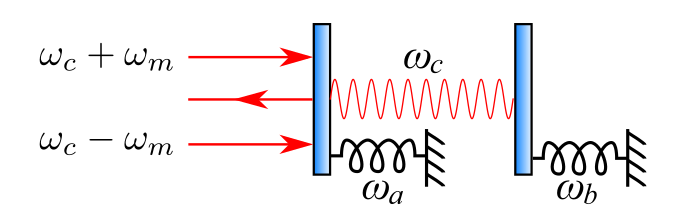
\includegraphics[width = 8 cm]{plots/plot_system.png}
		\end{figure}	

\end{frame}

% System and Hamiltonian II
\begin{frame}
	
	\frametitle{Introduction}
	\framesubtitle{System and Hamiltonian}
	
	Quantum optomechanics Hamiltonian
	\begin{figure}
		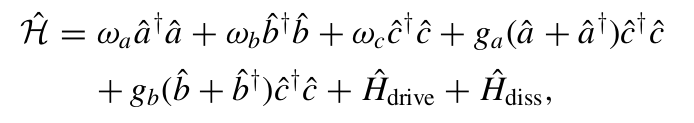
\includegraphics[width = 8 cm]{plots/hamiltonian_1.png}
	\end{figure}
	
	Under usual approximations, obtain the master formula 
	\begin{figure}
		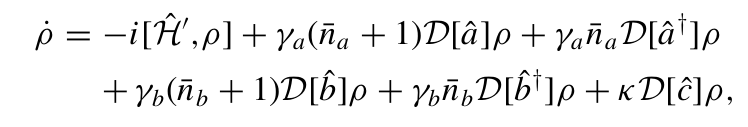
\includegraphics[width = 8 cm]{plots/master_eq_1.png}
	\end{figure}

	Being $\mathcal{H}' = \mathcal{H} - \mathcal{H}_{\textrm{diss}}$, and $\mathcal{D}[\hat{c}]$ the dispersive superoperator
	
\end{frame}

% Reservoir engineering I
\begin{frame}

	\frametitle{Reservoir engineering strategies}
	\framesubtitle{Linearized optomechanics}
	


\end{frame}

% Reservoir engineering I
\begin{frame}
	
	\frametitle{Reservoir engineering strategies}
	\framesubtitle{Bogoliubov operators}
	
	Define the {\color{blue}Bogoliuov} modes in terms of the modes $\hat{a}, \hat{b} \longrightarrow$
	\begin{figure}
		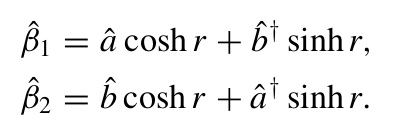
\includegraphics[width = 5 cm]{plots/bogoliubov_1.png}
	\end{figure}	

	Rotation with respect to a frame, being r the {\color{blue}squeezing parameter} 
	\begin{figure}
		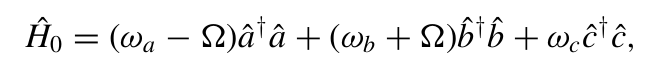
\includegraphics[width = 8 cm]{plots/hamiltonian_2.png}
	\end{figure}	

	Choice of $\Omega$ for non-trivial rotation of collective mechanical quadratures $\hat{X}_{\pm}$, $hat{P}_{\pm}$

\end{frame}

% Reservoir engineering II
\begin{frame}
	
	\frametitle{Reservoir engineering strategies}
	\framesubtitle{Squeezed modes}
	
	2-mode squeezed state defined by $|r> = S_{2}(r) |00>$
	\begin{figure}
		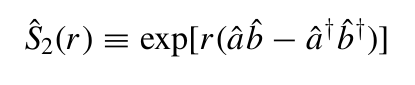
\includegraphics[width = 5 cm]{plots/2_squeezed_mode.png}
	\end{figure}	

	Such that $\hat{\beta}_{1}$ and $\hat{\beta}_{2}$ are the two-mode squeezed state with squeezing parameter $r$

	\begin{figure}
		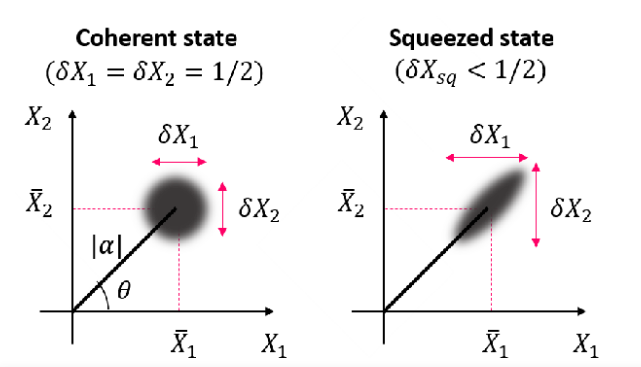
\includegraphics[width = 7 cm]{plots/plot_squeezed.png}
	\end{figure}
	
\end{frame}

% Reservoir engineering III
\begin{frame}
	
	\frametitle{Reservoir engineering strategies}
	\framesubtitle{Squeezed modes}
	
	\begin{itemize}
		\item i) Two cavity modes to independently cool the Bogoliubov modes (beam splitter $\hat{\beta}^{\dagger}_{i} \hat{c}_{i}$)
		\item ii) Couple the cavity to one Bogoliubov mode, and then this to the other via $\hat{\beta}^{\dagger}_{1} \hat{\beta}_{2}$ and the this to the other one
		\item iii) Couple the cavity to sum of the Bogoliubov modes , then the sum to the difference . Again, beam splitter interaction $\hat{\beta}^{\dagger}_{\textrm{sum}} \hat{\beta}_{\textrm{diff}}$ allows diff to cool.
		\begin{align}
			\hat{\beta}_{\textrm{sum}} = \frac{1}{\sqrt{2}}(\hat{\beta}_{1} + \hat{\beta}_{2}) \nonumber \\
			\hat{\beta}_{\textrm{diff}} = \frac{1}{\sqrt{2}}(\hat{\beta}_{1} - \hat{\beta}_{2}) \nonumber
		\end{align}
	\end{itemize}

	Cooling $\hat{\beta}_{\textrm{sum}}$ and $\hat{\beta}_{\textrm{diff}}$ is equivalent to cool $\hat{\beta}_{1}$ and $\hat{\beta}_{2}$ given $<\hat{\beta}^{\dagger}_{\textrm{sum}} \hat{\beta}_{\textrm{sum}}> + <\hat{\beta}^{\dagger}_{\textrm{diff}} \hat{\beta}_{\textrm{diff}}> = <\hat{\beta}^{\dagger}_{1} \hat{\beta}_{1}> + \hat{\beta}^{\dagger}_{2} \hat{\beta}_{2}$

\end{frame}

% Reservoir engineering IV
\begin{frame}
	
	\frametitle{Reservoir engineering strategies}
	\framesubtitle{Hamiltonian}
	
	Hamiltonian in terms of the Bogoliubov modes
	\begin{figure}
		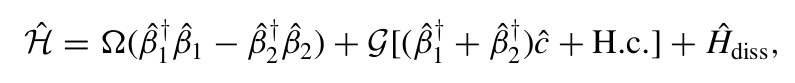
\includegraphics[width = 8.5 cm]{plots/hamiltonian_3.png}
	\end{figure}	
	
	where $\Omega$ is the effective frequency and $\mathcal{G}$ an effective coupling.
	
	Written in terms of the original operators,
	\begin{figure}
		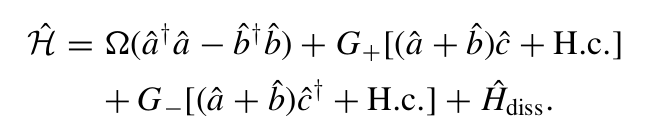
\includegraphics[width = 7.5 cm]{plots/hamiltonian_4.png}
	\end{figure}

	with couplings related by $\mathcal{G} \equiv \sqrt{G_{-}^{2} - G_{+}^{2}}$ and $\tanh r \equiv = G_{+}/G_{-}$

\end{frame}

% Implementation I
\begin{frame}

	\frametitle{Implementation}
	\framesubtitle{Different cases}
	
	Hamiltonian is already implemented in conventional optomechanical setups. Focus on regime $|G_{+}|<|G_{-}|$
	
	\begin{itemize}
		\item Two-tone driving ($g_{a} = g_{b}$)
		\item Four-tone driving ($g_{a} = g_{b}$)
		\item Case similar ($g_{a} \sim g_{b}$)
	\end{itemize}	
	
	(...)

\end{frame}

% Implementation - 2 tone driving
\begin{frame}

	\frametitle{Implementation}
	\framesubtitle{2 - tone driving}
	
	Single photon coupling rates equal $\longrightarrow$ cavity drive tones at $\omega_{c} \pm \omega_{m}$
	
	\begin{figure}
		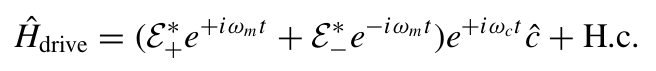
\includegraphics[width = 7 cm]{plots/hamiltonian_2_tone.png}
	\end{figure}

	\begin{columns}
		
		\column{0.5\textwidth}
		
		\begin{figure}
			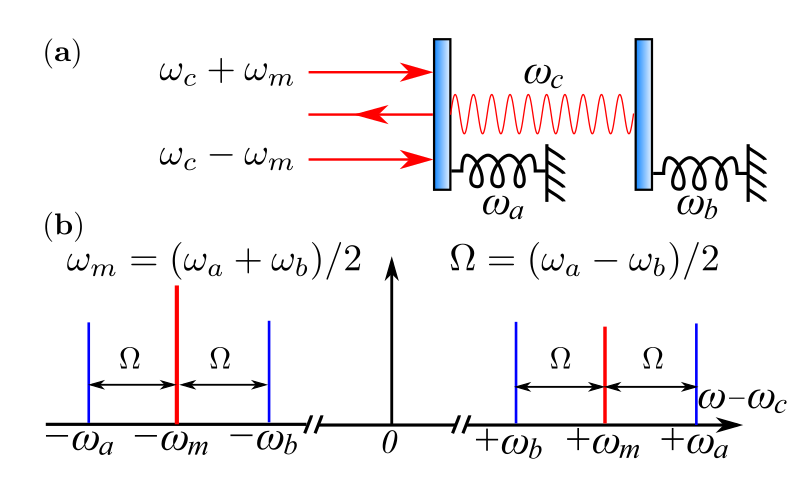
\includegraphics[width = 7 cm]{plots/plot_2_tone.png}
		\end{figure}	
		
		\column{0.45\textwidth}
		
		\begin{itemize}
			\item Interaction picture with respect to $H_{0}$
			\item Find the steady state amplitudes at the sidebands
			\begin{figure}
				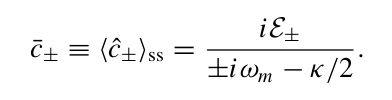
\includegraphics[width = 5 cm]{plots/ss_2_tone.png}
			\end{figure}
			\item Assumptions used (...)
		\end{itemize}
		
	\end{columns}

\end{frame}

% Implementation - 4 tone driving
\begin{frame}
	
	\frametitle{Implementation}
	\framesubtitle{4 - tone driving}
	
	Couplings unequal $\longrightarrow$ driving tones applied with detuning of $\Omega$ from the sidebands $\omega_{c} \pm (\omega_{a} - \Omega)$ and $\omega_{c} \pm (\omega_{b} + \Omega)$
	
	\begin{figure}
		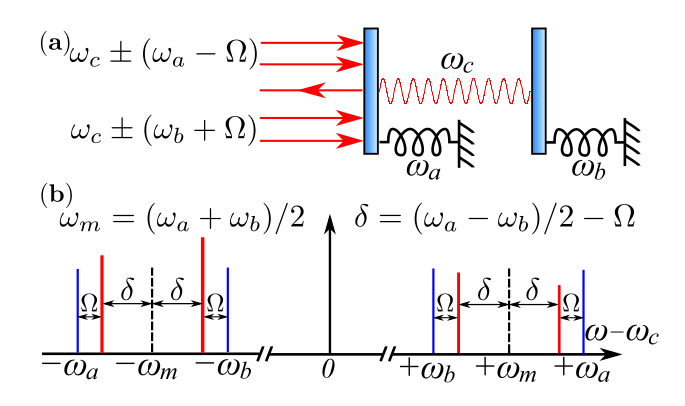
\includegraphics[width = 7 cm]{plots/plot_4_tone.png}
	\end{figure}	
	
	\begin{figure}
		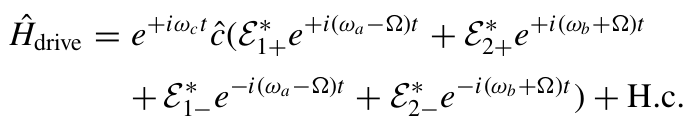
\includegraphics[width = 8 cm]{plots/hamiltonian_4_tone.png}
	\end{figure}

\end{frame}

% Implementation - 4 tone driving
\begin{frame}
	
	\frametitle{Implementation}
	\framesubtitle{4 - tone driving}
	
	Couplings unequal $\longrightarrow$ driving tones applied with detuning of $\Omega$ from the sidebands $\omega_{c} \pm (\omega_{a} - \Omega)$ and $\omega_{c} \pm (\omega_{b} + \Omega)$
	
	\begin{figure}
		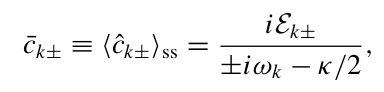
\includegraphics[width = 5 cm]{plots/ss_4_tone.png}
	\end{figure}

	\begin{itemize}
		\item Where we demand the strengths match as $\bar{c}_{1\pm} / \bar{c}_{2\pm} = g_{b} / g_{a}$
		\item Working in interaction picture with respect to Hamiltonian (4)
		\item Imprecision in the matching lead to add contributions as in Hamiltonian (14)
	\end{itemize}

	Condition $\gamma \ll \Omega \ll (\omega_{a} - \omega_{b})/2 - \gamma$, {\color{blue}sufficiently coupled} Bogoliubov modes and unwanted sideband processes have no effect.

\end{frame}

% Adiabatic limit I
\begin{frame}
	
	\frametitle{Adiabatic limit}
	\framesubtitle{Our system}
	
	\begin{itemize}
		\item Assume the system responds rapidly to mechanical motion $k > \Omega, G_{\pm}$, but still in $\omega_{a}, \omega_{b} \gg k$
		\item Get rid of the cavity operator $\hat{c} = -2i\mathcal{G}(\hat{\beta}_{1} + \hat{\beta}_{2})/k$\\
		\item Obtain adiabatically eliminated master equation
	\end{itemize}

	\begin{figure}
		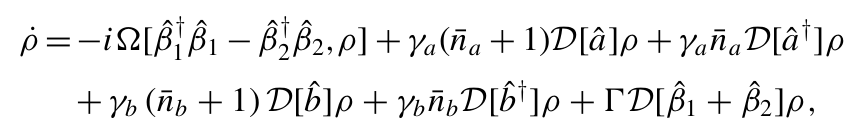
\includegraphics[width = 9 cm]{plots/master_eq_2.png}
	\end{figure}

	with optomechanical damping rate
	\begin{figure}
		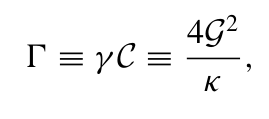
\includegraphics[width = 3 cm]{plots/optomechanic_dumping.png}
	\end{figure}

	Easy to obtain steady state, and to measure entanglement and purity.
	 
\end{frame}

% Adiabatic limit II
\begin{frame}

	\frametitle{Adiabatic limit}
	\framesubtitle{Entangled systems}

\end{frame}

% Adiabatic limit III
\begin{frame}
	
	\frametitle{Adiabatic limit}
	\framesubtitle{Entanglement}
	
	Entanglement criterion using Duan inequality 
	\begin{figure}
		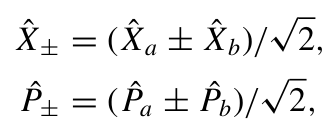
\includegraphics[width = 4 cm]{plots/entanglement_quad.png}
	\end{figure}	
	
	Where we introduced the quadrature modes as
	\begin{figure}
		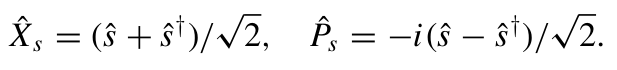
\includegraphics[width = 6.5 cm]{plots/entanglement_quad_2.png}
	\end{figure}

	Where we introduced the quadrature modes as
	\begin{figure}
		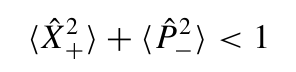
\includegraphics[width = 4 cm]{plots/entanglement_duan_criterion.png}
	\end{figure}

\end{frame}

% Adiabatic limit IV
\begin{frame}
	
	\frametitle{Adiabatic limit}
	\framesubtitle{Purity}
	
	Entanglement criterion using Duan inequality 
	\begin{figure}
		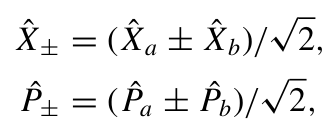
\includegraphics[width = 4 cm]{plots/entanglement_quad.png}
	\end{figure}	
	
	Where we introduced the quadrature modes as
	\begin{figure}
		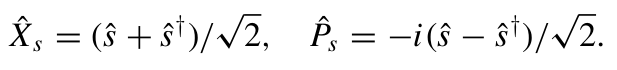
\includegraphics[width = 6.5 cm]{plots/entanglement_quad_2.png}
	\end{figure}
	
	Where we introduced the quadrature modes as
	\begin{figure}
		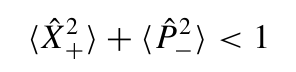
\includegraphics[width = 4 cm]{plots/entanglement_duan_criterion.png}
	\end{figure}

\end{frame}

% Adiabatic limit V
\begin{frame}
	
	\frametitle{Adiabatic limit}
	\framesubtitle{Entanglement}
	
	\begin{columns}
		
		\column{0.5\textwidth}
		
		\begin{figure}
			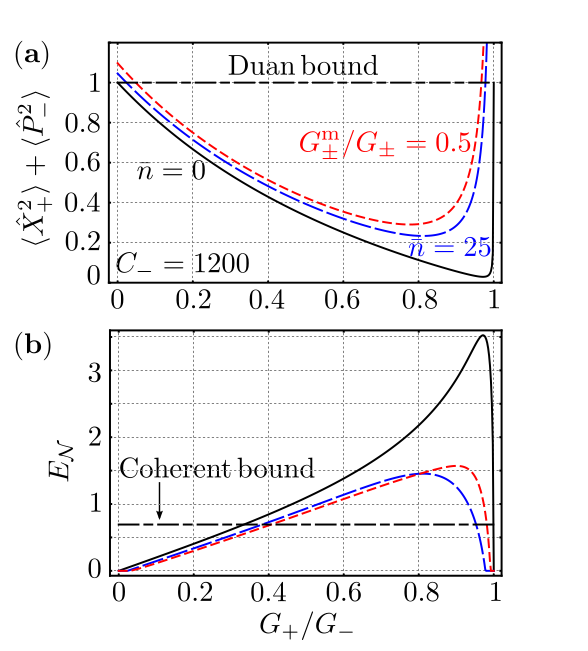
\includegraphics[width = 6 cm]{plots/plot_entanglement.png}
		\end{figure}	
	
		\column{0.65\textwidth}
		
		\begin{itemize}
			\item 1
			\item 2
			\item 3
		\end{itemize}
		
	\end{columns}

\end{frame}

% Adiabatic limit IV
\begin{frame}
	
	\frametitle{Adiabatic limit}
	\framesubtitle{Entanglement}
	
	\begin{columns}
		
		\column{0.5\textwidth}
		
		\begin{figure}
			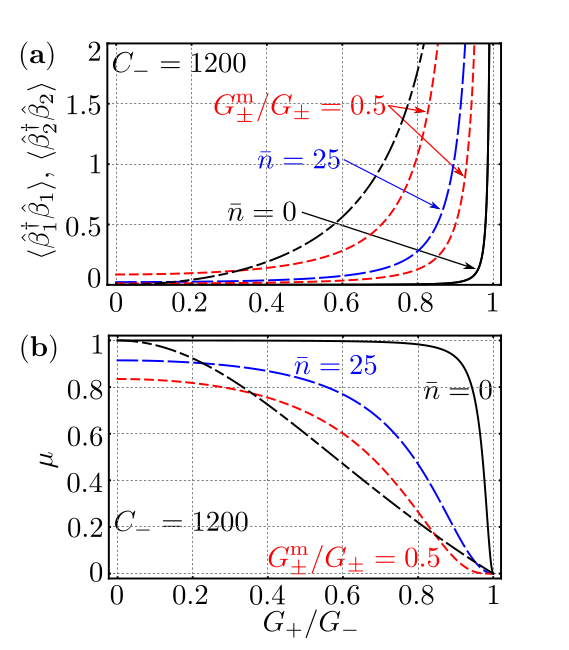
\includegraphics[width = 6 cm]{plots/plot_steady_state.png}
		\end{figure}	
		
		\column{0.65\textwidth}
		
		\begin{itemize}
			\item 1
			\item 2
			\item 3
		\end{itemize}
		
	\end{columns}

\end{frame}

% Time dependence
\begin{frame}

\frametitle{Time dependence}
\framesubtitle{time dependence}

	\begin{figure}
		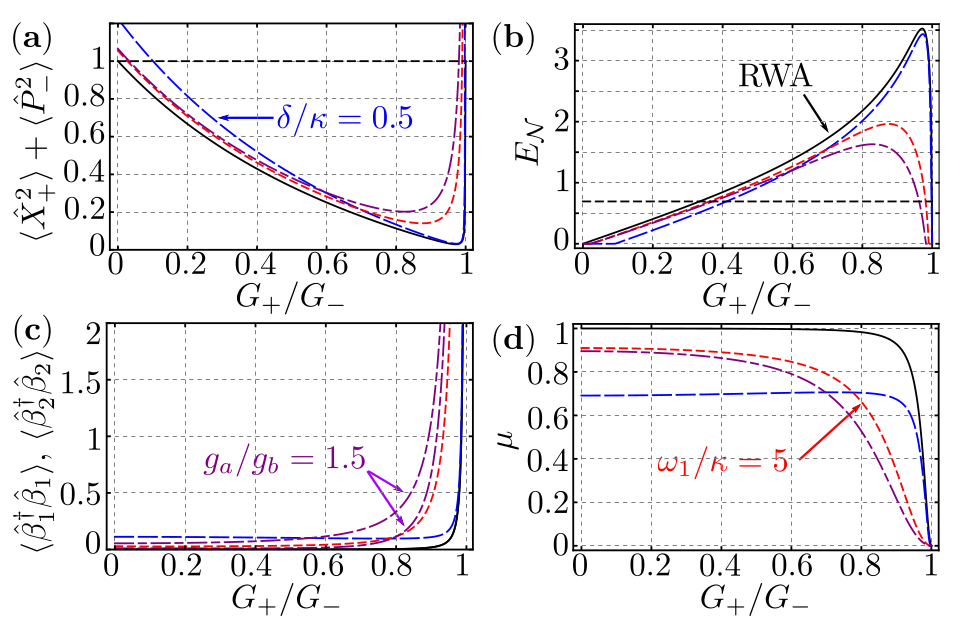
\includegraphics[width = 9 cm]{plots/plot_time_dependence.png}
	\end{figure}	
	
\end{frame}

% Experimental observability
\begin{frame}
	
	\frametitle{Experimental observability}
	\framesubtitle{Output spectrum}
	
	\begin{figure}
		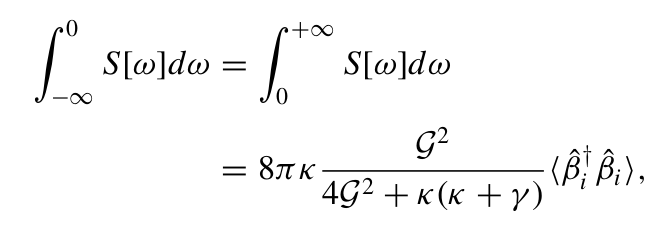
\includegraphics[width = 6 cm]{plots/spectrum.png}
	\end{figure}	

\end{frame}

% Experimental observability
\begin{frame}

\frametitle{Experimental observability}
\framesubtitle{Output spectrum}
	
	\begin{figure}
		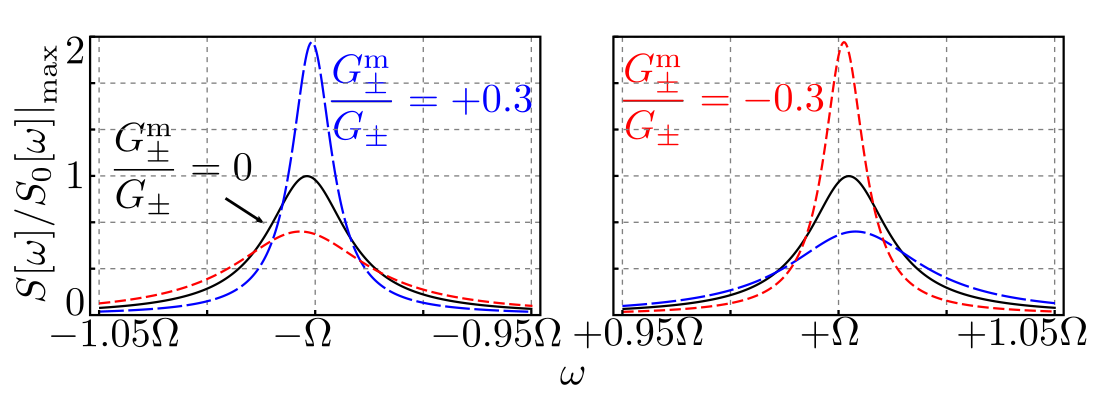
\includegraphics[width = 9 cm]{plots/plot_spectrum.png}
	\end{figure}	

\end{frame}

% Conclusions
\begin{frame}

	\frametitle{Conclusions}
	
	\begin{enumerate}
		\item Configuring a three-mode optomechanical system such as the steady state includes highly pure and highly entangled two-mode squeezed state.
		\item Symmetry on the steady-state makes it attractive for implementation of  continuous-variable teleportation protocols
		\item Problem of unequal single-photon optomechanical couplings solved by using four-tone driving scheme
		\item Proposal implementable for existing technology
	\end{enumerate}
		
\end{frame}
\end{document}